\section{GPU Architecture}
According to Flynn's taxonomy\cite{flynntax} computer architectures can be divided into
four types depending on the combination of a single or multiple instruction streams
with a single or multiple data streams:
\begin{itemize}
	\item{\textit{Single instruction, single data} (SISD)}
		is the simplest architecture since there is no parallelism at all.
		Examples for SISD include CPUs with a single core and embedded systems.
	\item{\textit{Multiple instruction, single data} (MISD)}
		is rarely used in practice since multiple instruction streams typically operate on separate data streams (see MIMD below).
		The most notable use of MISD is the use of multiple flight computers in the NASA space shuttle to provide redundancy.
	\item{\textit{Single instruction, multiple data} (SIMD)}
		is used to apply the same instructions to multiple data streams.
		This is useful for processing data in batches.
		GPUs are dedicated SIMD computers but modern desktop CPUs typically also
		implement some SIMD instructions as maligned by Linus Torvalds \cite{axv512}.
	\item{\textit{Multiple instruction, multiple data} (MIMD)}
		is the most general type of parallelism where multiple instructions can be executed
		in parallel on separate data streams.
		Multi-core CPUs as well as distributed systems function as MIMD computers.
\end{itemize}
While there are some tasks that are suitable for MIMD computers but not for SIMD computers (like compiling code)
the narrower range of tasks of an SIMD computer allows for hardware optimizations in its design.
As a simple example, consider that fetching and decoding instructions is not free;
some amount of logic needs to go into these steps which means that they take up precious die area.
If the same instructions are applied to multiple data streams
the amount of die area going towards fetching and decoding instructions decreases
while the amount of die area doing towards actually executing the instructions increases, thus increasing the throughput of data.

Modern GPUs in particular implement an architecture known as \textit{single instruction, multiple thread} (SIMT),
a subtype of SIMD that can be programmed similarly to multi-threading on CPUs:
the GPU executes multiple threads in parallel by executing the same instructions at the same time in each thread.
Branching instructions through the use of conditional statements or loops is supported by masking which threads get executed.
In the case of a conditional statement the GPU first executes the \textit{if} block with
all threads where the condition was evaluated as \textit{true};
threads where the condition was evaluated as \textit{false} are simply idling.
After executing the \textit{if} block the GPU executes the \textit{else} block in the same way but with an inverted mask.
Loops operate on the same principle as conditional statements with the mask being updated between iterations.
Of course, since branching instructions result in idle threads it should be kept to a minimum to maintain performance.
\begin{figure*}
	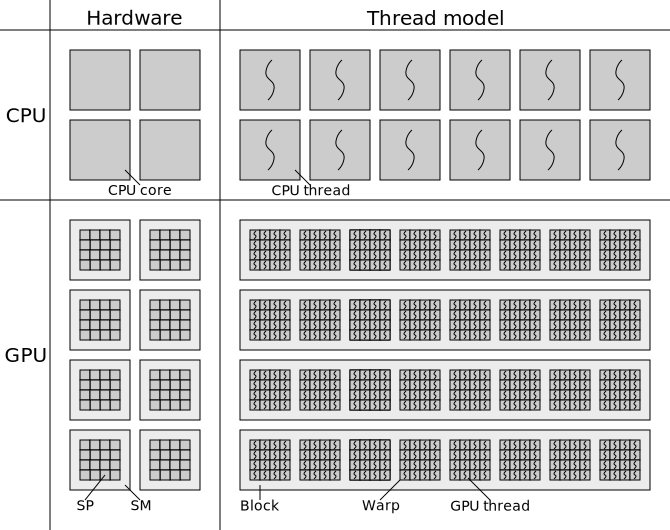
\includegraphics[width=\linewidth]{gpu-vs-cpu.png}
	\caption{
		Graphical representation of the analogy between hardware and thread model on CPUs and GPUs.
		Each CPU core can work on one thread at a time, so threads are managed individually.
		Each SM can work on multiple threads at once so threads are managed as warps.
		Warps are in turn grouped together as blocks.
	}
	\label{gpu-vs-cpu}
\end{figure*}

The difference in architectures between CPUs and GPUs is reflected in how they organize threads (compare figure \ref{gpu-vs-cpu}).
A CPU has one or more cores that execute threads one at a time, so threads are being managed as single threads.
A GPU has many so-called \textit{streaming multiprocessors} (SM) that in turn consist of many \textit{streaming processors} (SP).
The SPs on an SM synchronously run threads with the same instructions that are combined to a so-called \textit{warp}.
Each SM manages multiple warps which are in turn combined to \textit{blocks};
these are the units that are being assigned to an SM.

Each warp in a block executes the same code.
When a block is assigned to SM it begins to execute one of the warps in the block until no more work can be done on the warp
(e.g. because the warp needs to fetch data from memory).
The SM then performs a \textit{context switch} to another warp in the same block and continues to do work.
Ideally, the reason why one particular warp cannot do work will be resolved while the SM works on the other warps
(for example because the data arrives from memory).
In this case no time at all was spent waiting from the perspective of a single warp.
This practice is called \textit{latency hiding}.

It is important to note that unlike CPU cores, SPs do not have dedicated registers.
Instead they share the registers of the SM and these registers are \textbf{not} flushed upon a context switch.
This means that context switches between warps can be performed very quickly.
However, it also means that registers are shared between warps, reducing the number of available registers per warp.
Large warps can result in the eviction of registers used by other warps to memory, inducing latency on a context switch.

Due to the differences in their architectures multi-threading on a GPU
is utilized very differently when compared to multi-threading on a CPU.
On a CPU threads are very expensive and the overhead cost associated with
creating a large number of threads can outweigh the benefits gained from parallelism;
a common strategy for maximizing performance on a CPU is to create as many threads as there are logical CPU cores.
On a GPU however threads are extremely lightweight by comparison;
a common strategy for maximizing performance on a GPU is to create
many times more small threads than there are SPs to ensure that the GPU never runs out of work to do.

The difference in thread management described above reflects the difference in design goals between CPUs and GPUs.
CPUs are optimized for the execution of code that frequently branches (in terms of conditional statements or loops).
They have a large number of registers and large amounts of cache per CPU core to reduce the latency induced by memory accesses.
GPUs on the other hand are optimized for computational bandwidth.
They have a much larger number of comparatively slower SPs that are designed to run code with limited branching.
Because SPs have access to fewer registers and less cache than CPU cores GPUs are also more suited for code that
accesses data only once rather than many times.
